
% Added link to preamble
\documentclass[12pt]{article}
\usepackage[utf8]{inputenc}
\usepackage{blindtext}
\usepackage{graphicx}
\usepackage{tabularx}
\usepackage{authblk}
%\usepackage{natbib}
\usepackage{xcolor}
\usepackage{float}
\usepackage{amsmath}
\usepackage[english]{babel}
\usepackage{graphicx} % Required for inserting images
\usepackage[paperheight=16cm,paperwidth=12cm,textwidth=8cm]{geometry}
\usepackage[flushleft]{threeparttable,booktabs}

\usepackage[
        backend=biber,
        style=authoryear-comp,
        sorting=nyt,
        style=apa
    ]{biblatex}
 \addbibresource{references.bib}


 \geometry{
 a4paper,
 total={170mm,257mm},
 left=30mm,
 right=30mm,
 top=30mm,
 bottom=30mm
 }

% Keywords command
\providecommand{\keywords}[1]
{
  \small	
  \textbf{\textit{Keywords---}} #1
}

\graphicspath{{plot/}}



\addbibresource{}



\title{Social Class and Naming Patterns in Chile: Imitation and Differentiation}
\subti
\author{}
\date{February 2024}

\begin{document}
\maketitle

\begin{center}
    \textsc{Extended abstract} 
\end{center}

\section{Introduction}
The practice of naming offers a window into the symbolic and material mechanisms of boundary creation within societies. Unlike many cultural practices, name selection operates independently of direct economic or political constraints, providing a unique lens through which to explore motivations and desires that are less visible in other domains. This includes the longing for group belonging, the influence of socially structured aesthetic preferences, and more.
 \bigskip 

In the United States, racial distinctions are a prominent feature of naming patterns, particularly with the prevalence of uniquely African American names. Conversely, in European countries, names often reflect regional affiliations. More recently, naming practices have been interpreted as indicators of immigrant parents' desire to assimilate into their new countries.
 \bigskip 

However, the exploration of class-based naming patterns remains underdeveloped in existing literature. This article seeks to bridge that gap by examining the influence of class on naming trends in Chile throughout the 20th century. We uncover that naming practices are not only stratified by class but also reveal a nuanced process of class emulation and differentiation that operates from the top down. Through the lens of class-based naming patterns in Chile, we aim to illustrate the dynamic interplay of imitation and differentiation that underpins seemingly static symbolic dimension of social stratification. This case study sheds light on how names serve as markers of both individual identity and social hierarchy, revealing the complex interactions between personal choice, cultural influence, and social structure.
 \bigskip
 

In particular, our research tests the following hypotheses:

 
\begin{enumerate}
    \item Naming patterns in Chile are consistently stratified by social class across different periods.
    \item Names that are initially popular among the upper class become adopted by the middle and lower classes after a generation, suggesting a unidirectional flow of naming preferences. This trend may reflect the disproportionate influence of the elite in setting aesthetic standards, not merely as a marker of class aspiration but also due to their prominence in public life.
    \item In response to their names becoming more widespread, the upper class engages in two distinct strategies of differentiation: 
    
    \begin{enumerate}
       \item Innovation: The upper class tends to adopt novel names, thereby establishing new aesthetic norms.
       \item Recycling: The upper class revives names that have fallen out of common use but were popular in the past, reintroducing them into the naming repertoire
    \end{enumerate}

\end{enumerate}

\section{Methodology}

\subsection{Data}
The data on names used in this study comes from two main sources. First, we utilized the Chilean civil registry, which contains information on name, year, month, municipality (comune), and frequency for each registered name between 1920 and 2022. Secondly, we incorporated census data obtained from IPUMS, which has socioeconomic information from 6 Chilean censuses ranging from 1960 to 2017. Specifically, IPUMS provides occupation prestige scores for main income providers in each household. When two-income providers were present, we averaged their scores to get a household-level estimate. For single-income households, we used the sole provider's score \footnote{This data are available here: https://international.ipums.org/international/}.

\subsection{Variables}
Our goal was to analyze the socioeconomic dynamics in the diffusion of names across social classes over time. To do this, we first constructed a municipality-level socioeconomic status index for each available census year in IPUMS by taking the median occupation prestige score across households within each municipality. However, since the census socioeconomic information was only available for 1960, 1970, 1982, 1992, 2002 and 2017, we needed to extend this information to match the yearly name data we had from the Chilean civil registry spanning 1920 - 2022. To accomplish this, we carried out a data expansion process, where we took each municipality's socioeconomic index score for a census year and assigned it to a span of 5 years before and after that census. For example, each municipality's prestige score calculated for the 1960 census would be applied to the years 1955-1965 within that municipality. Through expanding the census prestige scores in this manner to stretch across gaps between census years, we were able to construct a complete, matching socioeconomic index at both the municipality and name level for the full set of years covered by the name frequency data (1920-2022). Ultimately, this process gave us 65 years of socioeconomic variability to analyze diffusion patterns over time.
\bigskip

With the municipal socioeconomic indexes covering the full period of interest (1920-2022), we constructed a name-level index weighted by the number of occurrences of that name in each municipality and year. More specifically, we took all municipal value-frequency pairings for a name and calculated a weighted average to obtain its corresponding historical socioeconomic index. Additionally, we categorized names into socioeconomic quintiles over time based on these indexes. Constructing sequences of quintile transitions for each name between 1960-2021 enables us to visually inspect and analyze shifts of names between different socioeconomic strata using sequencing techniques. The rationale behind dividing into 5 classes is to capture more granular movements that may not be visible using coarser divisions (e.g. low/middle/high).

\subsection{Descriptive strategy}


\begin{figure}[H]
\begin{center}
    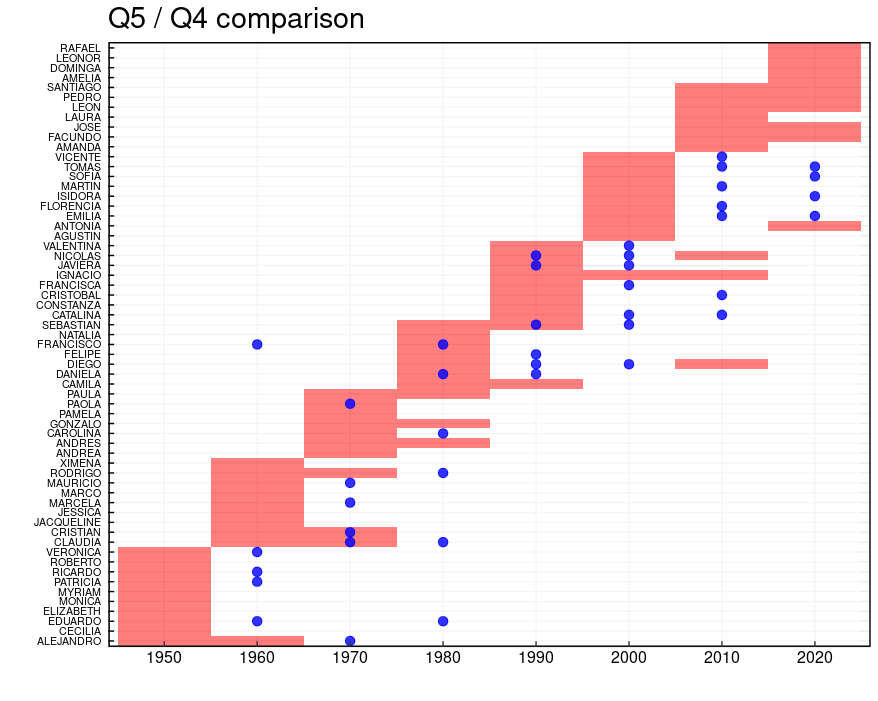
\includegraphics[width=12cm]{plot/q5_q4_comparison.png}
    \caption{Overlap top names (n=10) between Q5 and Q4 by decade}
    \label{fig:new_names}
\end{center}
\end{figure}

\begin{figure}[H]
\begin{center}
    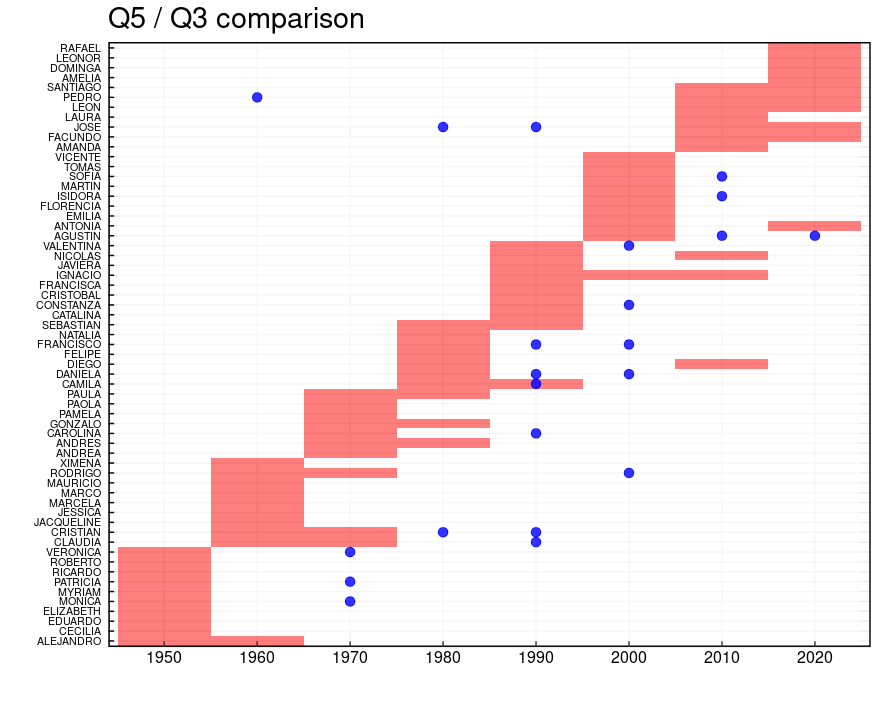
\includegraphics[width=12cm]{plot/q5_q3_comparison.png}
    \caption{Overlap top names (n=10) between Q5 and Q3 by decade}
    \label{fig:new_names}
\end{center}
\end{figure}

\begin{figure}[H]
\begin{center}
    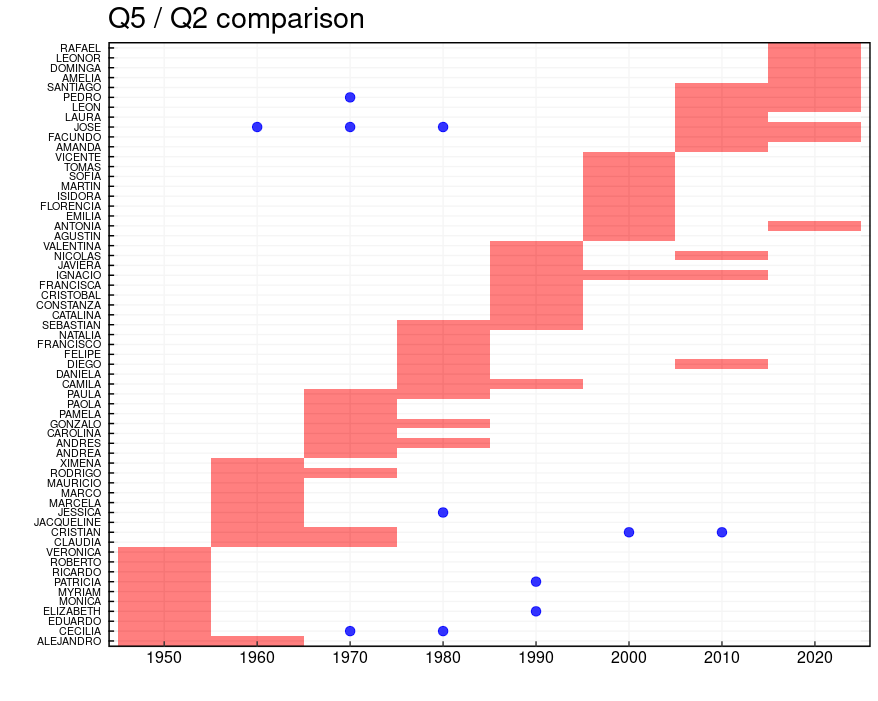
\includegraphics[width=12cm]{plot/q5_q2_comparison.png}
    \caption{Overlap top names (n=10) between Q5 and Q2 by decade}
    \label{fig:new_names}
\end{center}
\end{figure}

\begin{figure}[H]
\begin{center}
    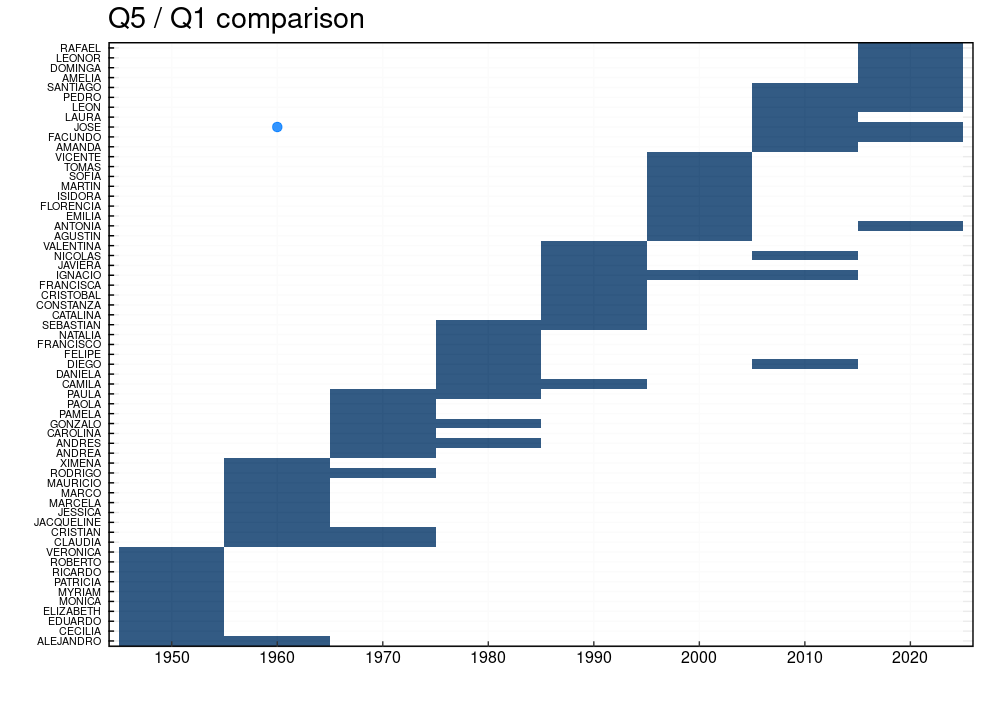
\includegraphics[width=12cm]{plot/q5_q1_comparison.png}
    \caption{Overlap top names (n=10) between Q5 and Q1 by decade}
    \label{fig:new_names}
\end{center}
\end{figure}



\begin{figure}[H]
\begin{center}
    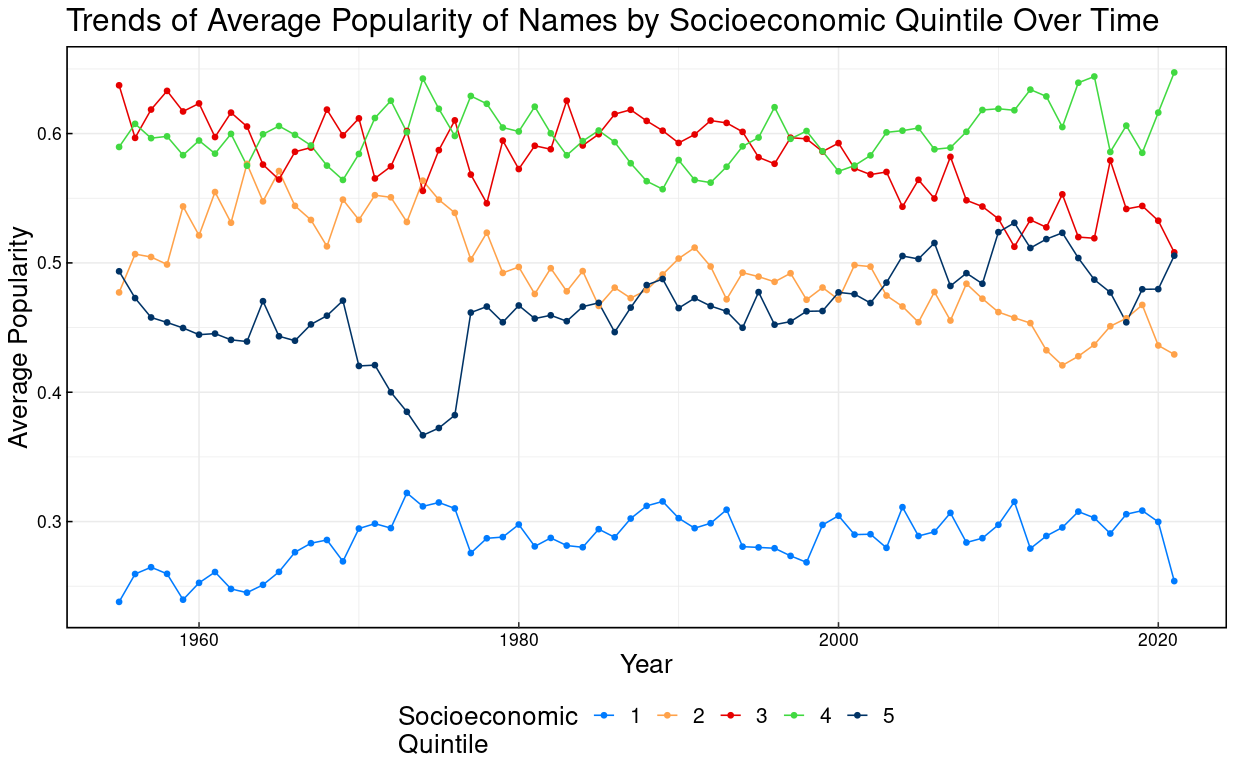
\includegraphics[width=15cm]{plot/p3.png}
    \caption{Trends of popularity by class}
    \label{fig:new_names}
\end{center}
\end{figure}

\begin{figure}[H]
\begin{center}
    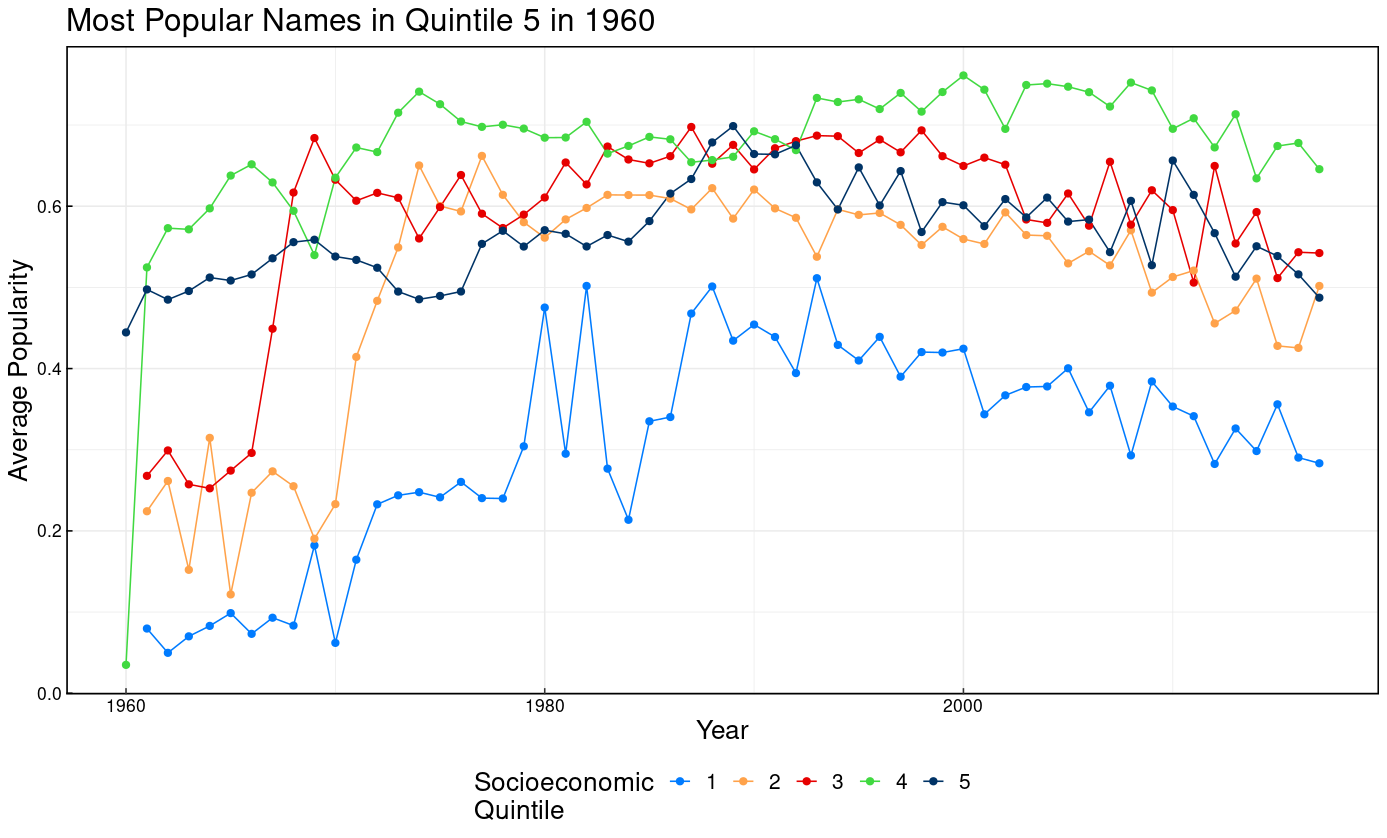
\includegraphics[width=15cm]{plot/p4.png}
    \caption{Trends of popularity by class}
    \label{fig:new_names}
\end{center}
\end{figure}


\begin{figure}[H]
\begin{center}
    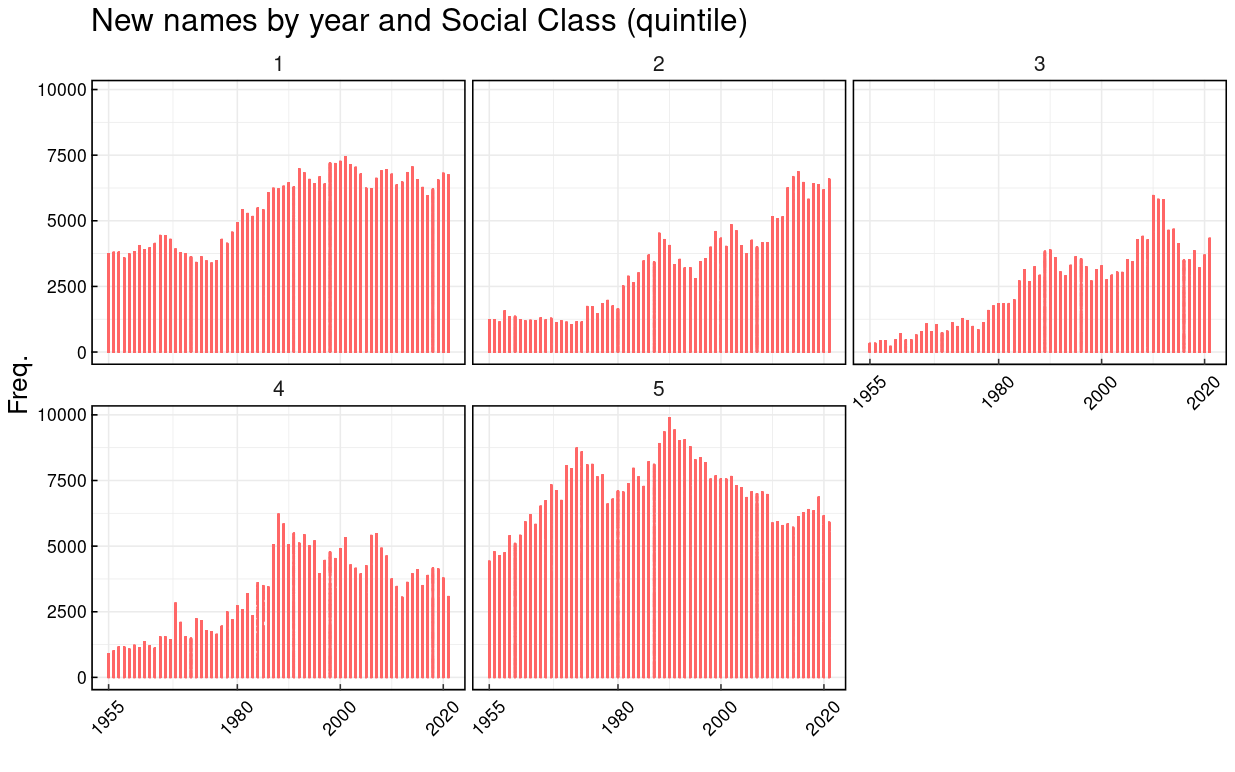
\includegraphics[width=15cm]{plot/p1.png}
    \caption{New names by year and social class}
    \label{fig:new_names}
\end{center}
\end{figure}


\begin{figure}[H]
\begin{center}
    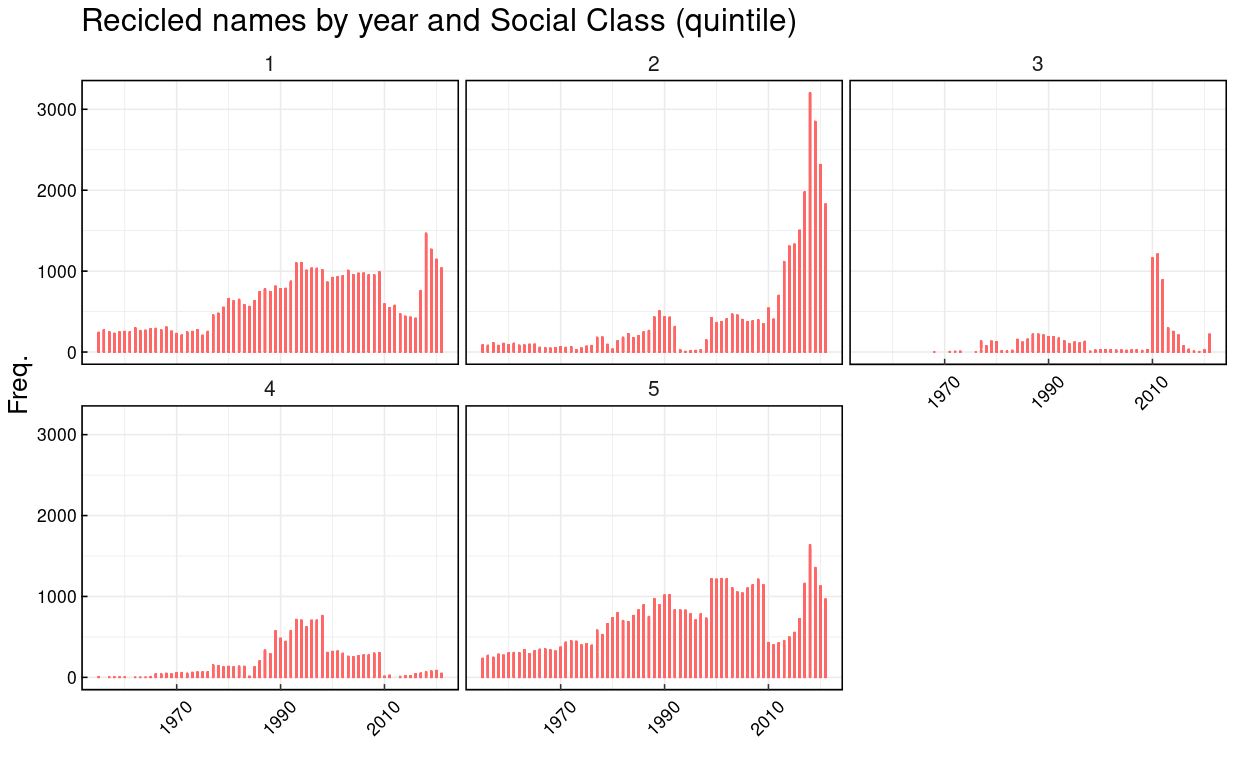
\includegraphics[width=15cm]{plot/p2.png}
    \caption{Recicled names by year and social class}
    \label{fig:new_names}
\end{center}
\end{figure}



\end{document}
